\section{偏移与速度佶计}
\label{sec:3.6}

我们经常会同时面鞍倾角、炮检距及速度未知这三种复杂情况,告速度已知时,双平方
根方程提供了一个颇有吸引力的解决难题之途径。可是当速度朱知时,可就把人难住了,采
用上一节中所述那样的速度估计姓理办法吧,可它却又是假设没有倾角的情形。在这一节
中,我们将建立一神界面存在倾角时进行速度估计的方法。

\subsection{倾角时差校正---Sherwood的“魔鬼”方法}
\label{sec:3.6.1}

倾斜地层与水平方向的交角为$\alpha$时,Levin关于该倾斜层的反射旅行时间$t$的表达式为
(见\ref{sec:3.2}节)
\begin{equation}
t^2v^2=4(y-y_0)^2sin^2\alpha + 4h^2cos^2\alpha
\label{eq:ex3.6.1}
\end{equation}

在炮检距与时间的空间$(h,t)$内,这是一支双曲线。以$cos\alpha$为比例系数将速度$v$放大,
可使这时距曲线同无倾角情形下的时距曲线完全相同\footnote{
以$v/cos\alpha$代替$v$时,即得这种结果。---译者
}。常规处理办法就是沿这种曲线进行
叠加和速度分析,它常常能有满意结果。有时,结果却不令人满意,因为倾角不婊空间的单
值函数,例如,断层面附近将会存在绕射,这时它们是所有倾斜同相轴的叠加结果,每个同
相轴强度一般均比反射要弱。在同一位置上可以存在许多同相轴倾角,这会使速度沽计和叠
加受到干扰。

原则上,叠前偏移---它是完整的双平方根方程的某类实现方法---可以解决这种普遍
性问题,但是,从何处取得用于偏移方程中的速度呢?尽管仅在涉及小角度时,偏移对速度
有点不灵敏,而当所涉及的是广角时,偏移对速度就变得比较灵敏了。

应当考虑一下偏移处理能否与速度估计处理混合使用。J.W.C. Sherwood(1976)曾
经指出偏移与速度估计这两种处理究竟应该如何混合使用。应当把时差校正分为两部分考
虑。一部分与炮检距有关,即正常时差校正(NMO);另一部分则与倾角有关,这后一部
分处理在概念上是新颖的。Sherwood将该种与倾角有关的处理描述为一类滤波处理,但他
并未提供方法实现的细节。他把他的处理方法称作Devilish(
“魔鬼”方法),这个词是“dipping-event velocity inequalities licked”(倾斜同相轴速度不等量修正)的缩写。以后
Yilmaz更为实用性地把该种处理称为叠前局部偏移,但是最后终究还是把这种处理直接称为
倾角时差校正(dip moveout or
DMO)。我们将首先看一下Sherwood所得结杲,然后讨论
Rocca的倾角时差校正概念模型,最后是对两种概念上有区别的处理方法进行定量说明。

\begin{figure}[H]
\centering
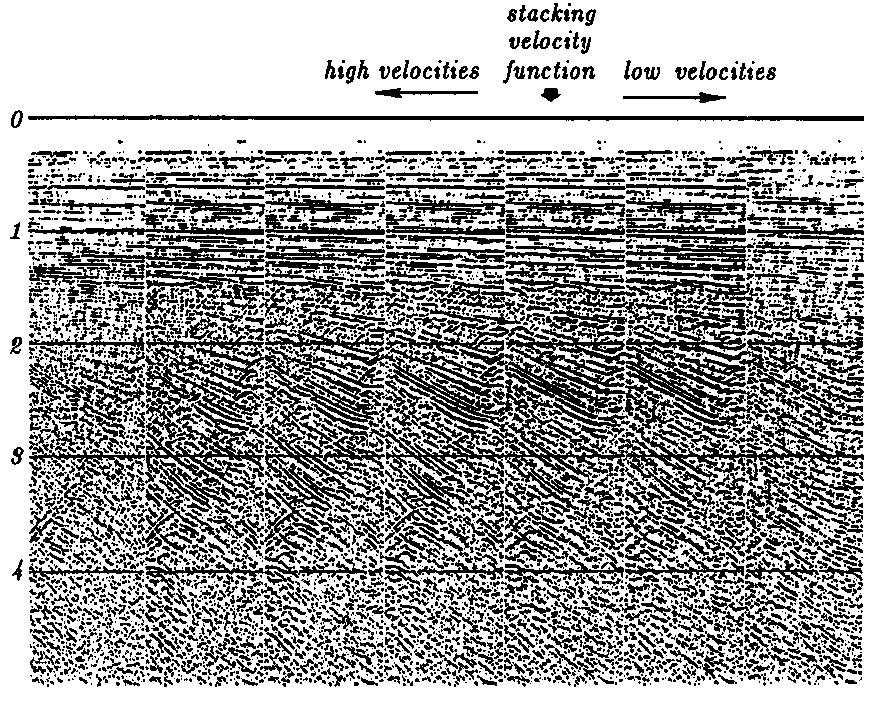
\includegraphics[width=0.65\textwidth]{vdmo/digicon}
\caption[digicon]{常规叠加速度扫描(Digicon公司提供)}
\label{fig:vdmo/digicon}
\end{figure}

图\ref{fig:vdmo/digicon}是叠加剖面的一小部分,这一部分在图中重复了若干次,每次采用的叠加速度
是不同的。要注意图中的特点,采用低速时,水平同相轴占优势;采用高速时,陡倾斜同相
轴占优势。在应用Devilish校正之后,像从前一样重新将数据叠加,结果如图\ref{fig:vdmo/rocca}所示,
这时叠加速度不再与倾角有关了。这意味着,在Devilish校正处理之后,测定速度能够无需
考虑倾角了,换句话说,所有各种倾角的同相轴对始终如一的相同速度都起作用,而不是每
一种倾斜同相轴各自预承心一种不同的速度。因此,Devilish这种校正处理对于具有相交同
相轴的资料理应能够提供更佳的速度,从而我们也就可以期望得到更好些的最终叠加结果。

\begin{figure}[H]
\centering
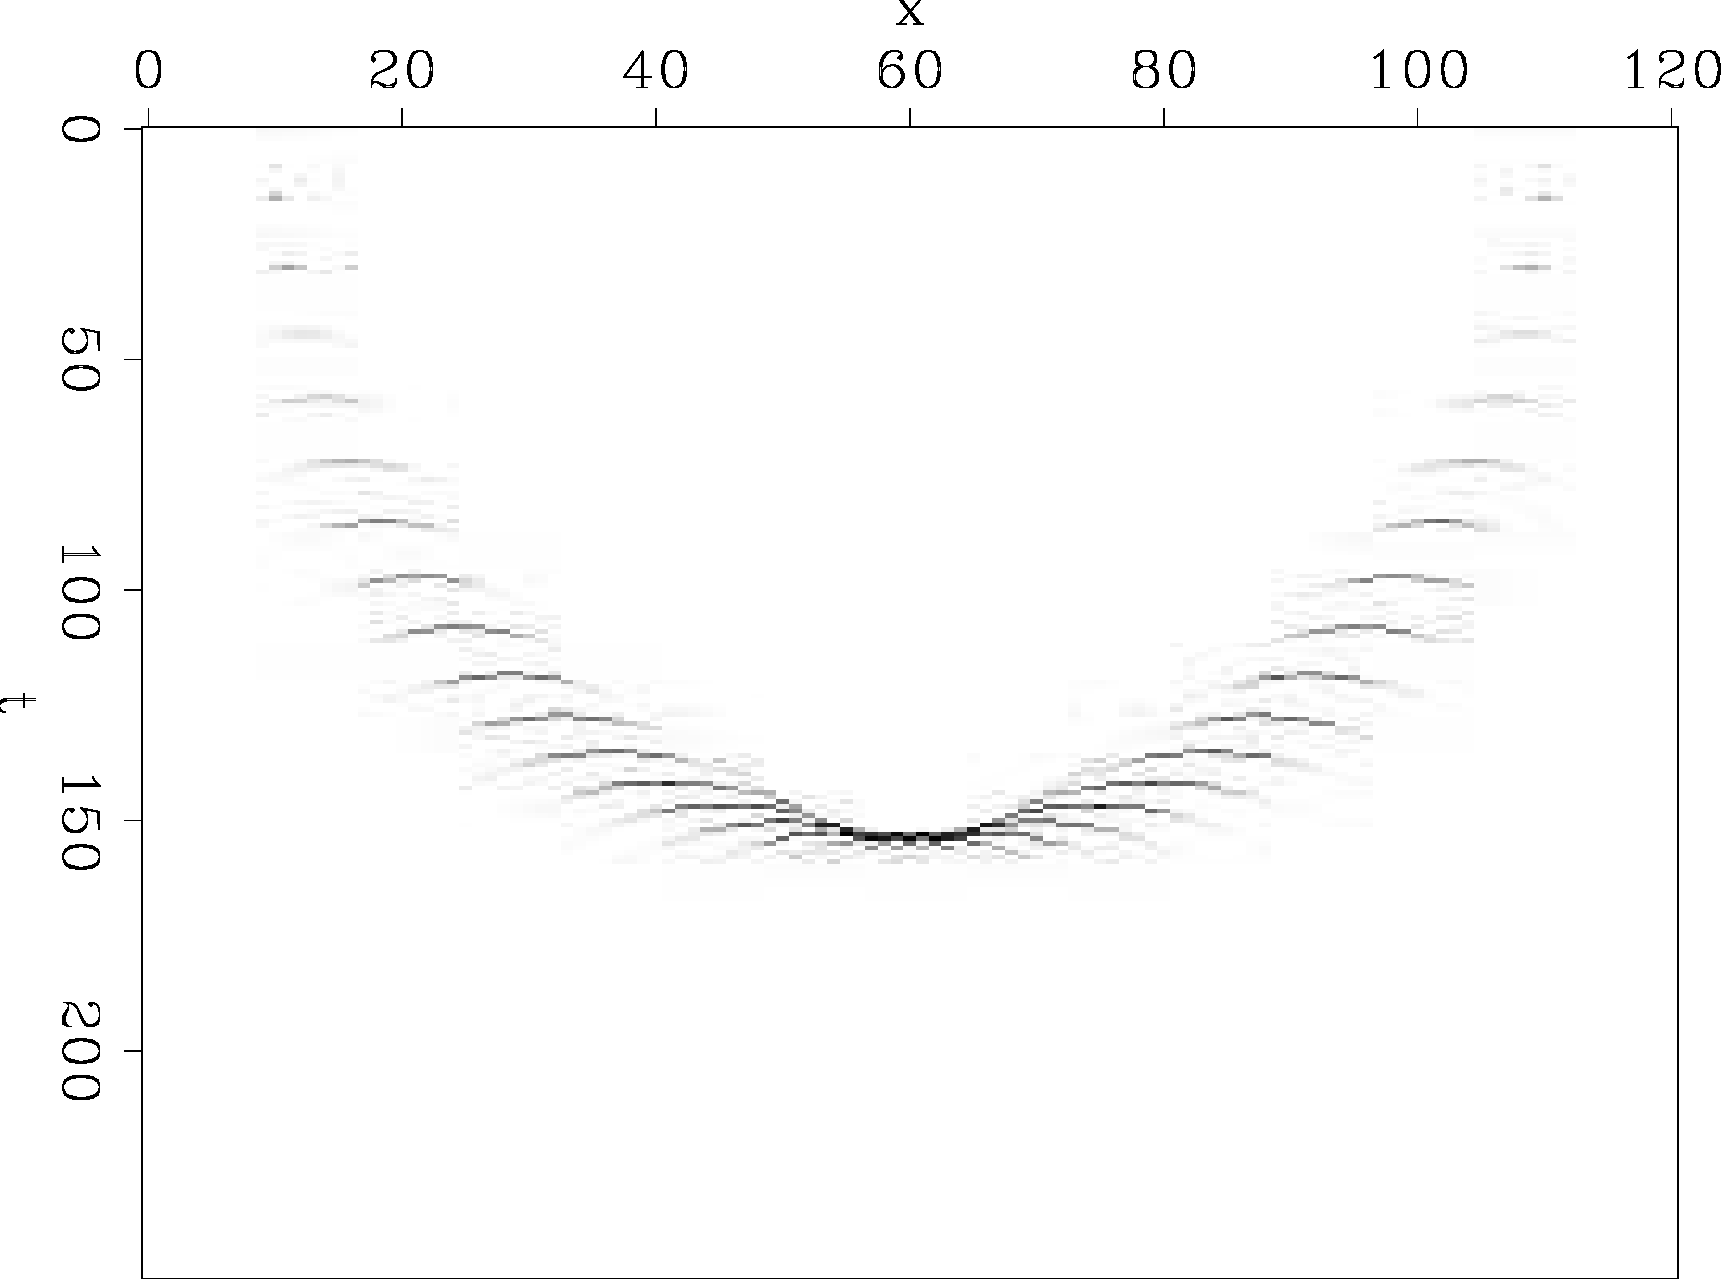
\includegraphics[width=0.65\textwidth]{vdmo/rocca}
\caption[rocca]{Rocca叠前局部偏移算子就是一种双曲线叠加,各该双曲线之顶点均位于半椭圆上。
将Rocca算子遍及中心点应用于共炮检距剖面,就可将该剖面转换为零炮检距剖面。
(据Gonzalez)}
\label{fig:vdmo/rocca}
\end{figure}

\subsection{Rocca的扫描算子}
\label{sec:3.6.2}

Fabio Rocca为Sherwood的倾角校正方法建立了一种概念清晰明确的摸型,现在用图
\ref{fig:vdmo/rocca2}来阐明Rocca的叠前局部偏移算子(prestack partial-migration operator)的概念。
试想像有一种在某个特定点$(t_0,y_0)$上含有一个脉冲函数的共炮检距剖面$P(t,y,h=h_0)$。其中,$t$为反射时间,
$y$为中心点坐标,$h_0$是该剖面所相应的固定炮检距。由于只有
$(t_0,y_0)$一个点上才有反射脉冲,这种资料所暗示的地层模型应是一个形状如半椭圆的反
射面,炮点在该椭圆的一个焦点上,接收点位于另一焦点上。根据这种地层模型,采用正演
模拟方法可作出一个相应的零炮检距剖面来,就是说,将半椭圆上的每一点扩展成双曲线,
即可得出零炮检距剖面。将共炮检距偏移和零炮检距绕射这两种运算结合起来,就得出了
Rocca算子。

\begin{figure}[H]
\centering
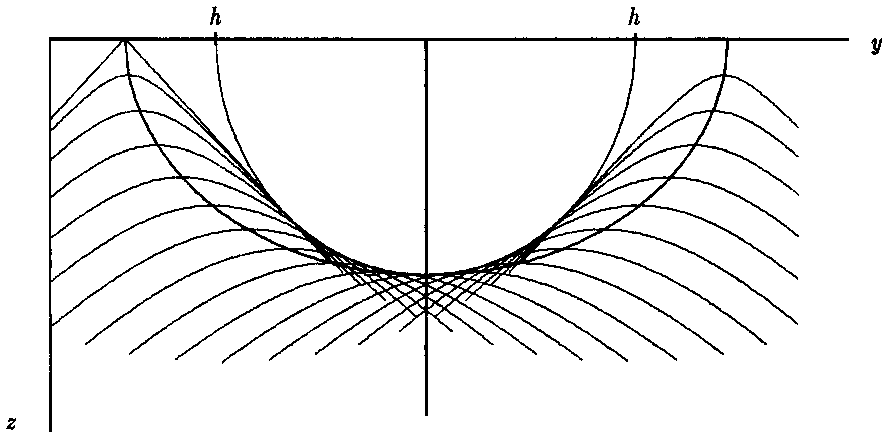
\includegraphics[width=0.65\textwidth]{vdmo/rocca2}
\caption[rocca2]{Rocca微笑曲线(据Ronen)}
\label{fig:vdmo/rocca2}
\end{figure}

Rocca算子就是图\ref{fig:vdmo/rocca}中的密切曲线(curve of osculation),
即各双曲线彼此得到
増强之处的微笑曲线(smile-shaped curve)\footnote{
该曲线状似人们微笑时的嘴,是以得名。---译者
}。如在椭圆弧上处处作出如图\ref{fig:vdmo/rocca}所示的
许多双曲线,而不是在几个孤立的点上作双曲线的话,这时该密切曲线就会在图上成为仅有
可见的东西了(而且还使你看不出它是从何而来)。

Rocca微笑曲线弧所相应之旅行时间的解析表达式表明,该弧是位于图\ref{fig:vdmo/rocca2}所示的一
个扃椭圆的末端部分。我们将略去这个微笑曲线方程的导出过程,最终可证明该方程为
\begin{equation}
\frac{(y-y_0)^2}{h^2}+\frac{t^2}{t_0^2} 
\label{eq:ex3.6.2}
\end{equation}
从这十方程看,Rocca算子好像是同速度无关似的。其实,它并不完全如此,因为微笑曲线
是在满足$dt/dy=2/v$关系的点上才截止的。

Rocca算子把共炮检距剖面变换成为零炮检距剖面,这种变换过程达到两个目的:第
一,它完成正常时差校正;第二,它完成Sherwood倾角校正。沿共炮检距剖面的中心点坐
标轴进行如图\ref{fig:vdmo/rocca}所示的运算,只在一个时间$t_0$上得出零炮检距剖面作为输出。对于每一
个时间$t_0$必须设计出不同的Rocca算子,所有$t_0$值时得出的输出必须叠加起来。图\ref{fig:vdmo/dmopoint}所
示就是若干$t_0$值时的若干个Rocca微笑曲线之叠加结果。

\begin{figure}[H]
\centering
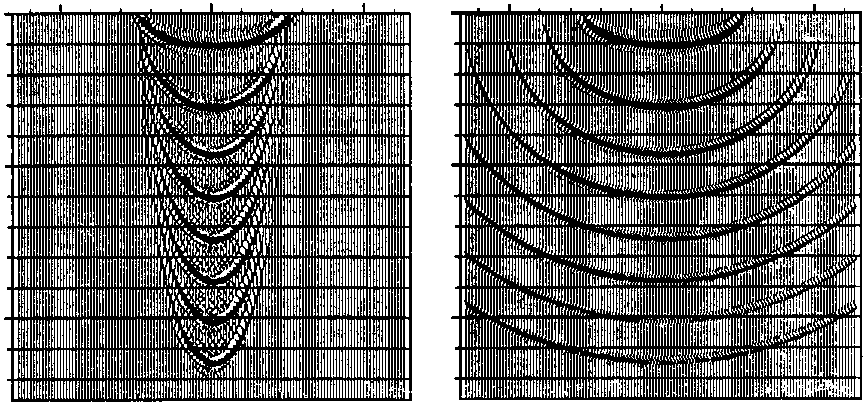
\includegraphics[width=0.65\textwidth]{vdmo/dmopoint}
\caption[dmopoint]{倾角时差校正之点源响应(左图)与共炮检距偏移扫描(右图)的比较(据Hale
)}
\label{fig:vdmo/dmopoint}
\end{figure}

从实用的观点看,这种算子特别有吸引力,因为对各个共炮检距剖面进行偏移处理时,
不是利用大而宽的椭圆进行大数据量处理,而只需要狭而小的Rocca算子。由图\ref{fig:vdmo/dmopoint}可
知,倾角时差校正算子\footnote{
文中所述倾角时差校正算子(dip moveout operator)、
Rocca微笑曲线、Rocca算子,Rocca叠前局部偏移
算子,密切曲线等等,大体均指同一类运算。---译者
}内的能量集中于该曲线底部附近很狭的范围内;在极限情形下,半
椭圆趋近于半圆,那就是说,在值较小的情形下,能量全部趋向底部。当所有能量集
中于底部一个点附近时,该Rocca算子实际上就变成一个$\delta$函数。在各炮检距均被校正为零
炮检距情形之后,根据正常时差剩余校正确定速度,然后再将数据叠加并偏移。

Rocca椭球体的扁度(narrowness
)在两种意义上有好处,从实用上说,它意味着在完
成速度估计和叠加以前,不需要将很多的中心点资料数据输入于计算机内存;更为重要的
是,由于算子所需的运算如此简洁紧凑,它确实不必对数据作大量运算。这点好处很重要,
因为运算是在完全已知速度之前的早期阶段完成的,所以有可能令人满意地选取区域性的恒
定值、例如取2.5公里/秒作为Rocca算子所需的速度值。

若有倾角时差校正算子的旅行时间曲线表达式,可能会有助于Kirchhoff积分求和型的
偏移扫描勉理,这将要求某些代数推导演绎,由此可导至Ottolini与Hale所建立算子牟身的
Fourier变换表现形式。

\subsection{Hale的共炮检距倾角时差校正}
\label{sec:3.6.3}

Hale(1983年)求出了对共炮检距剖面进行运算的倾角时差校正之Fourier变换表达形
式。参阅下表所列各定义方程:
\begin{table}[!ht]
\centering
\ttfamily
\small
\begin{tabularx}{\textwidth}{|Y|Y|Y|}
\hline
正常时差校正(NMO)& $t\rightarrow t_n$ & $t=\sqrt{t_n^2+4h^2/v^2}$\\
\hline
Levin正常时差校正& $t\rightarrow t_0$ & $t=\sqrt{t_0^2+4h^2cos^2\alpha/v^2}$\\
\hline
倾角时差校正(DMO)& $t_n\rightarrow t_0$ & $t=\sqrt{t_0^2-4h^2sin^2\alpha/v^2}$\\
\hline
\end{tabularx}
\end{table}
将倾角时差校正(DMO)方程代入正常时差校正(NMO
)方程中,就得出Levin正常时差校正方程\footnote{
$t$为反射时间,$2h$为炮点至检波点的炮检距,$v$为地层速度,$\alpha$为地层倾角,$t_0$为中心点(炮点与检波点之间的中心
点)下之界面的双程垂直时间(垂直深度$vt_0/2$)。若炮点位于上倾方向,检波点位于下倾方向,则炮点下界面的
双程垂直时间为$t_0-2hsin\alpha/v$;检波点下之界面双程垂直时间为$t_0+2hsin\alpha/v$;,由此可知,时间$t_n$为上述两种垂直时间的几何平均值。---译者
}。

要利用上表中的倾角关系方程,需知地层倾角$\alpha$,该倾角可由零炮检距剖面测定。在
Fourier空间内的零炮检距剖面上,该倾角的正弦为$vk_y/2\omega$,其中$k_y$为沿中心点坐标$y$的空
间波数;为强调这种测定仅应用于零炮检距剖面,我们总将$\omega$写为$\omega_0$,即
\begin{equation}
sin\alpha = \frac{vk_y}{2\omega_0}
\label{eq:ex3.6.3}
\end{equation}



%
% 切除函数往往是以r为变量的一维函数,其中\footnote{h为炮检距,t为时间.------译者},$r=h/t$。
% 既切除大r值时的数据也切除小r值时的数据,其原因如下所述。
%
% 在小r值时,炮点附近仍然可发现有能量存在,诸如水或泥块坠落所形成的影响,或者
% 低速地滚波所形成的干扰能量。
%
% r值大时,则存在与初至有关的问题。在这种情形下,正常时差拉伸最大而且对速度极
% 敏感。这初至往往称作首波或折射波。从野外观测看,首波就是一种其旅行时间表现为距离
% 之线性函数的波。就理论上考虑,针对分层介质很容易对首波作出解释。首波具有沿一地层
% 边界面作水平传播的射线。在实际现象中,首波可以弱于或者是强于反射波,首波强于反射
% 波可以用反射波作三维分布而首波仅作二维分布这个事实来解释。
%
% 可以把切除楚理看作是用零值迸行加权。为产生最有利的叠加效果,可以选择更普遍性
% 的加权办法。完善的分析肯定应将干扰噪音和截断影响考虑在内,我们权且作一个简化分析
% 吧,它可导出最基本的加权函数。
%
% 一般我们是沿双曲线遍及所有炮检距进行求积。考虑三维问题时则与此不同,你这时实
% 际是希望遍及一旋转双曲面进行求积,假设该双曲面是呈径向对称的,按炮检距h的大小对
% 被积函数进行加权,就使得通常的线性积分能够模拟出遍及旋转双曲面的积分结果
% \footnote{这是必须迸行加权处理的第一个理由.所谓沿双曲线的积分,实即正常时差校正并叠加;所罚沿旋转双曲面求
% 积,就是考虑球面扩散影响时的叠加。因此,必须按炮检距的大小,成比例地对叠加道(所谓被积函数)进行加权,校正
% 该种影响,这时的叠加处理(所谓的线性积分)结果,才能消除三维情形下的能量扩散。直接了当地说,进行加权处理的
% 第一个理由就是必须对波阵面球面扩散影响进行适当的补偿。}。叠加
% 前要按炮检距h的大小对数据进行按比例放大,还有第二个原因,那就是在零炮检距附近能
% 获得的速度信息不多,这些记录道的时差很小而在远炮检距时则可获得很多速度信息,这些
% 记录道的比值比较大
% \footnote{这是必须进行加权处理的第二个理由。浅显地说,近炮点记录道时差小,因而速度分辨率低;远炮点记录道时差
% 大,速度分辨率高。但是近炮点记录道振幅强,而远炮点记录道因能量衰减而振幅弱,采用以叠加方法为基础的速度分析
% 时,将因此而主要是反映近炮点记录道的作周和影响,降低了速度分析的精度。因此必须按炮检距的大小而成比例地加权
% 放大记录道辐值,使得近炮点与远炮点记录道的振幅在叠加中发挥同等作用。这种加权处理,对远度谱而言,可提高速度
% 分辨率;对叠加处理来说,可提高叠加效果和质量。----译者}。
%
% \subsection{NMO(正常时至校正)方程}
% \label{sec:3.5.4}
%
% 在任一已知记录资料的深度范围之内,地层速度变化范围可达2倍左右,是很典型的情
% 形。这样一来,对于以毕达哥拉斯关系为基础的分析方法就得需要重新加以考虑砑究了。在
% 实际处理中,总是采取在毕达哥拉斯关系中插入一个随时间而变的速度这种办法来处理随深
% 度而变的速度(有关的经典参考文献见Taner与Koehler[l969]的论文,它包括有许多颇有
% 助益的细节讨论)。尽管计算正确的非双曲线时差校正并不困难,很多还是采用这种近似。
% 让我们看一看倒底是如何在数学上将速度函数$v(z)$同正常时差联系起来的。设共中心点道
% 集之一记为$P(h,t)$,正常时差校正将该CMP道集转换为某一地层模型$Q(h,z)$
% \begin{equation}
% Q(h,z)=earth(z)\times const(h)
% \label{eq:ex3.5.1}
% \end{equation}
% 实际上,$Q(h,z)$终究还不是$h$的恒定函数,它还只是我们所欲达到的目标。
%
% 可以把正常时差校正处理看成是一种简单的复制过程。这点在概念上很容易想像,它就
% 是把$(h,t)$平面上的每一个点复制拷贝到$(h,z)$平面上的适当位置。可将这一类拷贝过程记为
% \begin{equation}
% Q[h,z(h,t)]=P(h,t)
% \label{eq:ex3.5.2}
% \end{equation}
% 这么拷贝时,必须小心避免在$(h,z)$平面上留下一些空洞
% \footnote{正常时差校正值需为时间采样间隔$\Delta t$的整涪数,但应校正的值不一定诒为其整数倍。在校正处理过程中,
% 超过整数倍之余值累积到等于一个$\Delta t$值时,须进行内插。所谓“空洞”,即应内插之处。----译者}。
% 最好是对$(h,z)$输出平面
% 内的每一个点迸行扫描,从而从$(h,t)$平面内找出其在$(h,z)$平面内产生该空洞的根
% 源。利用某种动校正时间表$t(h,z)$,可采取下列拷贝处理过程,对数据加以时差校正
% \begin{equation}
% Q[h,z(h,t)]=P[h,t(h,z)]
% \label{eq:ex3.5.3}
% \end{equation}
%
% 如采用本书的术语,时差校正处理的输入数据$P(h,t)$被称作CMP道集(共中心点道
% 集),而输出数据Q则被称作CDP道集(共深度点道集)。
%
% 在实际处理中,生成该旅行时间表的第一个步骤是把深度变量变成一垂直旅行时间变
% 量$\tau$。所以,所要求的表是$t(h, \tau)$,为得到位于$(h, \tau)$
% 的输出数据,你得在位置$(h,t)$
% 上取输入数据。产生这种时间表的最直接而可靠的途径,看来得按$z$的步长向下推迸。实际
% 也就是按$\tau$的步长向下推进,并沿射线追踪。那就是说,你要针对Snell参量$p$的各种固定值,
% 采用对下列两项方程遍及$\tau$迸行积分的办法根据$v(\tau)$计算出必$t(p,\tau)$和$h(p,\tau)$来
% \begin{equation}
% \frac{dt}{d\tau}=\frac{dz}{d\tau}\frac{dt}{dz}=v\frac{1}{vcos\theta}=\frac{1}{\sqrt{1-p^2v(\tau)^2}}
% \label{eq:ex3.5.4}
% \end{equation}
% \begin{equation}
% \frac{dh}{d\tau}=\frac{dz}{d\tau}\frac{dh}{dz}=vtan\theta=\frac{pv(\tau)^2}{\sqrt{1-p^2v(\tau)^2}}
% \label{eq:ex3.5.5}
% \end{equation}
% 在式\ref{eq:ex3.5.4}与式\ref{eq:ex3.5.5}中,$dt/dz$和$dh/dz$的表达式均是以射线为基础而不是以波阵
% 面为基础。给定了$t(p,\tau)$和$h(p,\tau)$,为消去$p$然后求出$t(h,\tau)$,需要进行叠代及内插方
% 法。这听上去挺难处理的---事实确实也是如此---因为在大角度时通常存在有到达反射
% 同相轴中部的首波,不过,一旦完成了这项工作,你就能存该表而多次重复利用它了。各
% 时距曲线在大炮检距上出现交叉分支现象,推动了以波动方程为基础的速度分析方法的建
% 立,最大的速度灵敏度正是出现在传统的双曲线假设初单一初至假设均不成立的那些地方。
%
%
% \subsection{线性性质与统计估计}
% \label{sec:3.5.5}
%
% 波动方程数竭处理方法具有的线性性质使柺我们能将数据集分解成儿部分,对每部分分
% 别地处理,然后将它们重新组合,所得结果同未作分解时处理所得结果相同。
%
% 例如,设把共中心点道集分成两部分,比如,分成近记录道部分A和远记录道部分B。
% 令$(A,0)$表示各远记录道均已置零的共中心点道集,$(0,B)$可以是该道集的另一拷
% 贝,其中各近记录道均已置零。我们可将$(A,0)$向下延拓,然后再独立地将$(0,
% B)$向下延拓。在各自完成向下延拓之后,可将$(A,0)$与$(0,B)$相加起来。我们可以轮流地
% 暂停延拓,就统计姓理作出某神考虑,然后选择用某种加权函数把它们组合起来。图\ref{fig:vdmo/decomp}
% 所示为三个记录道组成的数据集被分解成三个数据集,每道就是一个数据集,图中的半圆是
% 各记录道单独进行向下延拓时的扫描路径,每个半圆都通过零炮检距,给岀已适当展乎、经
% 过正常时差校正之后的记录道\footnote{这就是本书所谓的“波动方程时差校正”,实际就是叠前偏移。 ---译者}。
%
% \begin{figure}[H]
% \centering
% 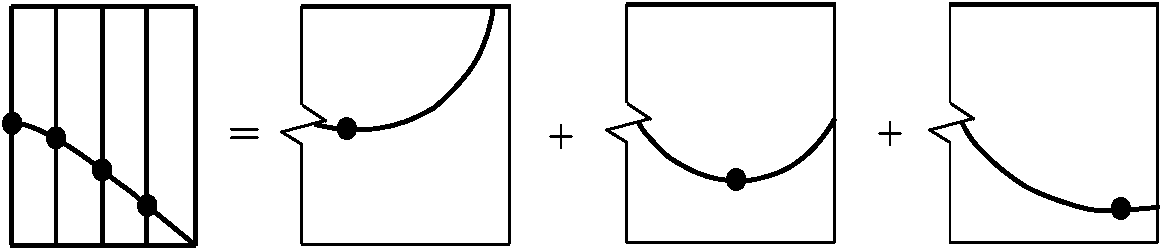
\includegraphics[width=0.65\textwidth]{vdmo/decomp}
% \caption[decomp]{三个记录道组成的共中心点道集按各记录道分解成三部分
% 左端,资料中的豚冲经过内插处理,可描绘出一双曲线轨迹。右端,各数据点均扩展成偏移半圆,
% 各半圆均通过位于双曲线顶点的零炮检距}
% \label{fig:vdmo/decomp}
% \end{figure}
%
% 采用加权函数这神思想,极端不同于我们先前进行分析的风格,它代表一种干扰识别的
% 概念,这是我们始终忽略了的在所有科学分析中都很重要的某种东西,那就是统计方法!是
% 什么因素要求选择一种加权函数呢?因素有很多,信噪比是起作用的一种因素;某些记录道
% 可能受噪音干扰或缺失,也是因素.当斟酌最终显示形式时,必须考虑人的感觉能力,并且
% 需要压缩动态范围,以便很小的值也能被发现.不但在明显易见的$(h,t)$空间内,而且在
% 频率域、倾角域或者在可能使波场过于超出均衡状态的任何其他空间内,都必须考虑动态范
% 围的压缩问题。
%
% 分解数据集有许多种方法,究竟选择何者,这决定于你的统计模型和你是否愿意使处理
% 重复进行许多次。也许数据道集的几部分不应该按其炮检距$h$来分解,而只应按它们的$r=h/t$
% 的值来分解。显然,要考虑的问题是很多的。
%
% \subsection{共中心点道集的横向内插与外推}
% \label{sec:3.5.6}
%
% 因为记录道数目不充分而产生了一些涉及到共中心点道集的实际矬理问题。截断问题便
% 是因检波器电缆只有一定长度并非长达遍及地震波传播之距离而发生的实际问题。图\ref{fig:vdmo/nmotrunc}
% 说明为什么电缆截断不但对波动方程方法,而且对常规的射线追踪和叠加方法也都是一个问
% 题。还有,假频问题便是因炮点与检波点彼此不是足够靠近而产生的实际问题。沿炮检距坐
% 标轴出现空间假频,它对波动方程方法的影响看来比对射线追踪方法的影响是个更为严重的
% 问题,原因在于正常时差校正降低了空间频率。因与检波器、电缆及地面耦合条件等实际问
% 题有关而形成的数据缺失空白,也常常会造成意外的困难。
%
% 本节将随同关于佶计缺失记录道的系统处理方法之讨论,一起解决这些问题。所述该项
% 技术,是斯坦福大学SEP科研项目(Stanford Exploration
% Project)目前正在发展的更
% 为一般性的缺失数据佶计处理程序系列中最简单的一种。
%
% 首先作正常时差校正,就是说,把双曲线时距曲线拉伸展平。首先遇到的问题是:必须
% 用什么速度作正常时差校正才行。为易于进行记录道内插,合适的时差校正速度应该属于道
% 集上占优势能量的那种速度。在给定的一 个数据集上,这秤速度可以在某些时间上
% 是一次波速度,而在另一些时间上是多次
% 波速度。需用这类无物理意义的速度的原因为:必须妥善地处理强同相轴,以便保
% 留较弱的一些同相轴。弱同相轴的截断影晌可作为“二阶问题”而忽略不计。通
% 常,实际问题是要在存在有沉积地层弱反射的背景上,将海水层之强同相轴压
% 制掉,尤其在高频时更需如此。原则上,
% 我们是能够在存在强P-P波的背景上搜寻
% 出弱P-SV波的。
%
% \begin{figure}[H]
% \centering
% 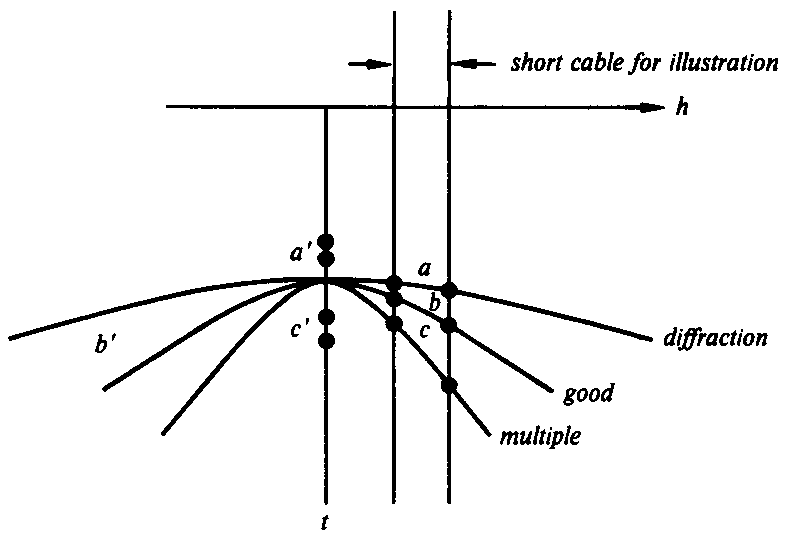
\includegraphics[width=0.65\textwidth]{vdmo/nmotrunc}
% \caption[nmotrunc]{以地层速度进行正常时差校正,可使良好同相轴上由电缆截
% 断的两点校正至良好位置,不引起作么间题•可是,绕射与多次
% 波的电缆截断点却校正至$a'$和$c'$,可能成为令人讨厌的问题。
% 这类说误所形成的干扰会造成畸变影响,使得根据共深度点叠加
% 求出波形时所作的精细复杂的时间序列分析全白费功夫了}
% \label{fig:vdmo/nmotrunc}
% \end{figure}
%
% 正常时差校正之后,残余能量应具有
% 很小的倾角,缺失数据之处当然除外,
% 这些地方用零值代替就迫使目前的数据在
% 空间波数域内成为宽频带了。为了改善我
% 们对于这种受到严重干扰的能量连续性之
% 视觉,我们使数据经过一稗可令高波数能量通过的"劣通"(badpass)滤波,诸如像\ref{sec:2.5}节
% 所讨论的高通递归倾角滤波
% \begin{equation}
% \frac{\frac{k^2}{-i\omega}}{a+\frac{k^2}{-i\omega}}
% \label{eq:ex3.5.6}
% \end{equation}
% 注意,这种滤波将大大地削弱具有小波数$k$的能量,即已经过适当时差校正的能量;另一方
% 面,在各缺失记录道附近,要注意波数纪或内的谱应是宽带的,因而这样的能量几乎是以单
% 位増益通过该“劣通”滤波的。
%
% 现在就从原有数据中减去“劣通”滤波的输出。这种减法要有选择地作,在存在记录数
% 据之处则什么也不减。这就完成了第一次叠代。然后,重复这些步骤和叠代,当在缺失记录
% 数据的位置上“劣通”滤波不再输出什么时,就最终达到了收敛。图\ref{fig:vdmo/missfil}所示是这种处理
% 的一个例子。
%
% 上述处理已忽略掉沿中心点方向存在有倾角的可能性,倾角影响要到\ref{sec:3.6}节才着手考
% 虑。
%
% 因为忽略了一个数据集也许会同时存在若干种速度的可能性,这种处理过程在应用方面
% 也是受限制的,为真正搞好这类扩展数据集的工作,可能需要有一个精确的模型以及像下一
% 节和\ref{sec:5.4}节中所讨论的速度谱的概念。
%
% \begin{figure}[H]
% \centering
% 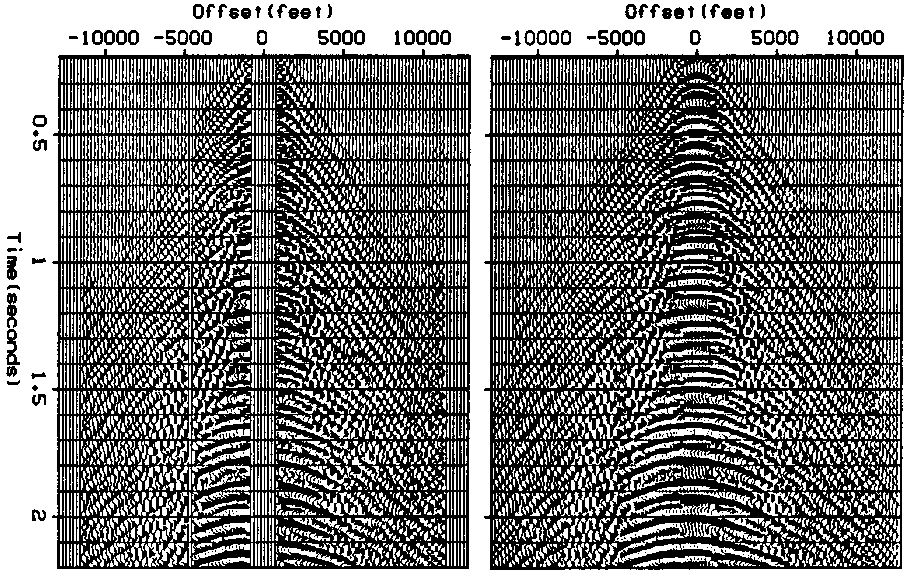
\includegraphics[width=0.65\textwidth]{vdmo/missfil}
% \caption[missfil]{左图:阿拉斯加地区有缺失空白道的野外记录;
% 右图:对上述记录进行递归空间滤波后的恢复结果。}
% \label{fig:vdmo/missfil}
% \end{figure}
%
% \subsection{速度空间的变换}
% \label{sec:3.5.7}
%
% 沿双曲线轨跡按各炮检距进行共中心点道集求和,把如此得到的一个叠加结果称作常速
% 叠加(constant-velocity stack
% )或CV叠加。可以把速度空间就定义为是一族CV叠加、
% 许多速度各自都对应于一个叠加。CV叠加是一种从炮检距空间至速度空间的变换,进行CV
% 叠加就是根据一个$(t,h)$空间的共中心点道集来形成一个$(t,v)$
% 空间的速度分布图形。
% 常规生产性的速度依计方法相当于增添有平方与归一化处理的CV叠加。诸如CV叠加这类的
% 续性变换一般都是可逆的,但是变换至速度空间是属于非常高维次的变换,48道而且每道有
% 1000个时间采样点,这就使该种变换成为48,000维的变换了。就目前的计算机技术而言,矩
% 阵有这么大是没办法用代数方法求逆的,然而,却有一些出色盼近似求逆办法可供选用。
%
% 对于酉矩阵(unitary matrix)来说,转置矩阵是等于逆矩阵的。
% 在波动传播理论
% 中,一个转置算子总是满意地近似于一个逆算子。Thorson(l984)曾经指出,对CV叠加的
% 转置运算就跟CV叠加本身没什么两样。要对CV叠加作转置运算,得从一个速度分布图形开
% 始作起,即从一个$(t,v)$空间中的图形作起。为形成某个给定炮检距A时的原始状态,首
% 先必须强使$(t,v)$图形中的每一个记录道恢复原来的正常时差;亦即,必须迫使同相轴从
% $(t,v)$图形中所具有的零炮检距时间$t_0$恢复到与给定炮检距$h$相应的时间上去。然后遍及
% 所有速度$v$将该种$(t,v)$
% 图形进行叠加,以产生该给定炮检距形下的地震记录。对所有
% 的待求炮检距的值A重复迸行上述恢复过程,即可恢复原来的共中心点道集。除了把时差
% 校正拉伸公式改变成对压缩进行补偿之外,对CV叠加进行转置运算的程序同CV叠加本身的
% 运算程序很相像。
%
% CV叠加的逆过程类似于倾斜叠加的逆过程或者Radon变换(见\ref{sec:5.2}节),就是说,CV
% 叠加差不多就是它本身的逆,不过,你需要改变一个符号,而且在最后阶段为了修饰$(t_0,v)$
% 空间的速度谱,还需要进行像$\rho$滤波那样的一稗滤波运算,至此才算结束了工作。正是
% 由于进行$\rho$滤波,才使逆CV叠加有别于CV叠加的转置。
%
% “转置”这个词是指矩阵转置。由于我们现在讨论的数据空间是二维的而一些算子却是
% 四维的,难于看出在这种情形下为什么适用“转置”这个字跟。但是,如果你愿意采用像
% \ref{sec:2.2}节中式\ref{eq:ex2.2.25}和式\ref{eq:ex2.2.26}那样的变换的话,
% 把这些二维和四维的对象表示成熟悉的一维和二维形式,那时你就会明白“转置”这个词完全是适用的。
% CV叠加所需要的$\rho$型滤波比普通的$\rho$滤波要稍微复杂一点---详情请参阅Thorson的论文.
%
% \begin{figure}[H]
% \centering
% 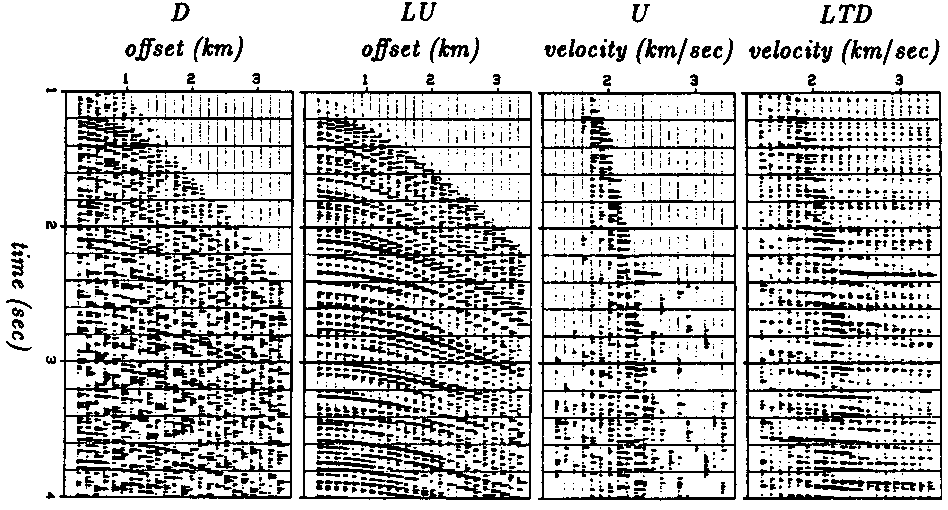
\includegraphics[width=0.65\textwidth]{vdmo/thor}
% \caption[thor]{左端图形D为墨西哥海湾地区的共中心点道集,第二个图形(LU)是第三
% 个图形(U)经过逆正常时差校正和叠加后得到重建数据,最后一个图形(LTD
% )是第一个图形(D)的CV叠加}
% \label{fig:vdmo/thor}
% \end{figure}
%
% 图3.5-7是Thorson的速度空间反演的实例。图形D为原始共中心点道集,其次一个图
% 形LU是速度空间的反变换结果,它是D的近似重建图象,其中双曲线同相轴比随机噪音恢
% 复得非常好,随机嗓音没有恢复得如此好是因为CV叠加中的速度范围限制取在水层速度与
% 3.5公里/秒之间。图形LTD是对D进行CV叠加之结杲,LTD再经$\rho$型滤波处理后得图形U,
% 图形LU就是U的转置CV叠加。
%
% 值得注意的是计算如LTD之类的速度谱时,需有大量计算量,必须对每一矜速度值来计
% 算CV叠加。下一节和\ref{sec:5.4}节中,将述及利用波动方程的速度识别方法,各科波动方程方法一
% 般比较节省计算量,不过它们的效果还不完全能对比。
%
% \subsection{$(z,t)$平面方法}
% \label{sec:3.5.8}
%
% 在$15^\circ$延拓方程$U_{zt}=-1/2vU_{hh}$中,对深度$z$进行比例标定或对速度进行标定,是没有
% 区别的。所以,以错误的速度进行向下延拓,可能就会向下延拓至错误的深度。
% Stephen M.Dohert(1975)就曾经在速度估计办法中利用过这种思想。参阅图\ref{fig:vdmo/doherty}。
%
% \begin{figure}[H]
% \centering
% 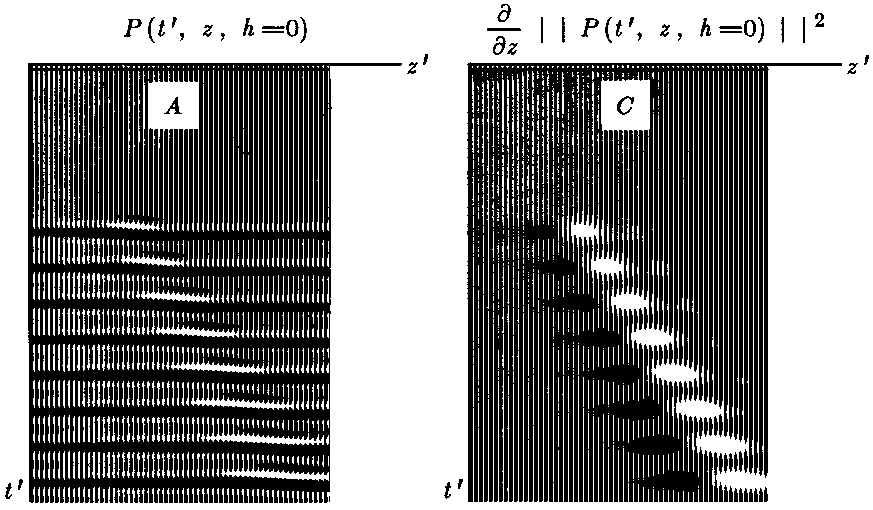
\includegraphics[width=0.65\textwidth]{vdmo/doherty}
% \caption[doherty]{零炮检距时的两种$(z,t)$平面显示。
% 地层模型为海水层之下有八个均匀分布的反射面,它们相应于$z=0$时,即未延拓时在$(h,t)$平面内的一
% 组双曲线。左边显示是零炮检距记录道,聚焦时的振幅极大尚非明显可见,但是相移是显著的。右边显示
% 是零炮检距记录道之包络对延拓深度$z$的导数,沿$z'=vt'$呈线性排列成行,相当显著(据Doherty
% )}
% \label{fig:vdmo/doherty}
% \end{figure}
%
% 这种思想是:按一个初始的速度模型实现向下延拓,然后在所有的旅行时间“深度”
% $\tau$上显示出作为$t'$之函数的零炮检距记录道.如果极大振幅出现在$t'=\tau$时,则你的初始速度
% 模型就是对的;如果极大值出现移动,那么在你能说明对下一次叠代应该采用什么速度之
% 前,你得分析一下才好。
%
% \subsection{将道集分解为高速分量与低速分量}
% \label{sec:3.5.9}
%
% 本节将定义一种处理过程,这种处理能够把共中心点道集的反射和折射全部划分为两部
% 分,一部分具有高于某种给定速度模型$\bar{v}(z)$的均方根速度,而另一部分则具有低于$\bar{v}(z)$的速度。
%
% 在作这样一秤分类之后,可以消除掉低速干扰。再不然,根据速度谱在相应地层速度处
% 应有峰值这科一般假设,可以通过叠代方法求忠地层速度。以后将会看到,利用按速度进行
% 数据分类这种方法所具有的线性性质和可逆性,还有可能进行各稗不同的数据内插、横向外
% 推以及其他统计处理方法。
%
% 处理办法很简单。开始时利用一个共中心点道集,将负值炮检距各道的数据均置零,然
% 后按照速度模型$\bar{v}(z)$把该道集向下延拓。具有小于$\bar{v}(z)$之速度的数据部分将为过偏移,
% 分布于从零炮检距至负炮检距;具有大于$\bar{v}(z)$之速度的数据部分则将为偏移不足,它们将
% 移向零炮检距但不会通过它。所以,低速部分位于负炮检距,而高速部分则位于正炮检距。
% 如果你希望的话,还可以将处理过程反向,使两部分回到原始数据空间。
%
% 显然,用一个阶跃函数乘该数据,可能会形成一些不受欢迎的绕射,可是不这么作,你
% 又没有指望能求出一种无限尖锐的速度截止滤波。显而易见,这时可以采取折衷的办法,用斜
% 坡函数来代替阶跃函数就能够减小这种虚假的绕射波。有一种使负炮检距A的数据置零的替代
% 办法是变换至波数频率域$(k_h,\omega)$内,然后在$k_h$与$\omega$之符号互异的两个象限内将数据均置零。
%
% 可惜,这种分类方法本身并不会提供速度谱。远离零炮检距$h=0$之处的能量未被聚焦,
% 而且同速度也并非明显有关。由于计算速度谱的需要,进一步推动了发展其他处理方法。
%
% \subsection{剖面上的反射首波}
% \label{sec:3.5.10}
%
% 追踪识别反射首波对一位叠加剖面解释人员来说是件常事。从观测现象上看,这只不过
% 是在时间剖面空间$(t,y)$内所见到的一种双曲线渐近线而已。从理论上说,它具有这样一
% 种射线:远离震源沿一水平分界面运动直至遇到某种不规则体、也许是遇到断层,它从那里
% 反射并返回至震源。反射首波有时称为折射反射(reflected
% refraction)。这种同相轴提
% 供了一种很容易的速度倍计方法,即从数据处理的观点看,像这样一种速度测
% 定方法是出乎意料的,因为自动处理方怯是在炮检距空间内提取所有的速度信息,许多解释
% 人员都愿意把这种空间保存在计算机内存中。当然,对于一个要加以追踪识别的反射首波,
% 必须提出一种特定地质环境的解释---这是一个散射体,其能量应强到足以使它的双曲线渐
% 近线明显可见。该点散射体还必须能量强得足以经受得住爆炸组合与检波器组合影响以及
% CDP叠加影响之典型的抑制作用。受到最高程度抑制的水层速度与地滚波速度,正是叠加剖
% 面上最经常见的那些速度(回想一下Larner条痕)。在\ref{sec:3.2}节中所示的共炮点剖面上已出现
% 过某些折射反射能量。
%
% 根据反射作出的速度估计都是反射点以上所有地层速度的平均结果,为提高速度的深度
% 分辨率,有必要减去不同深度水平的速度佶计结果(见\ref{sec:5.2}节);由于进行这种减法,就损
% 失了精度。所以,利用反射波求速度,很自然就得在精度与深度分辨率之间采取折衷办法。
% 另一方面,根据首波估计速度,在深度方面就自然具有高分辨率。
%
% 数据处理似乎忽略或轻视了反向散射传播的首波,然则它总能遇着并被加以利用。这种
% 状态必然事出有因,说不定这里还存在有某种潜在机会。从理论观点来看,Clayton的余弦
% 校正法已经证明过,在广角情形时,速度对炮检距的灵敏度和倾角对中心点的灵敏度出现了
% 相反的变化。但是在时间较大时,另一种因素的影响却变得明显起来了
% :即排列长度可能非
% 常之小于偏移双曲线的宽度。所以,尽管很容易在中心点空间内发现渐近线,可是在炮检距
% 空间内,排列末端上的时移却很小,难以检测。
%
% 有什么处理方法既能得益于反射的横向连续性、而又能加强而不是降低这种利用渐近线
% 进行速度测定的能力呢?就以高速度进行叠加为例说起吧,这时需利用下列思想:在任何深
% 度$z$上,频率波数域$(\omega,k_y)$内之时间剖面二维变换$U(\omega,k_y)$
% 的功率谱都应在损耗时差
% 参量$p(z)=k_y/\omega=1/v(z)$时出现截止。在功率谱$U*U$的图形中,或者更恰当地说,在倾角
% 谱的图形中,这种现象将表现为是深度之函数。或许在对待求速度进行倾角空间内的滤波之
% 后,就能够更好地用肉眼检查地震剖面本身了。
%
% 波场外推方程是一种全通滤波(all-pass filter),因此,为什么功率谱却是随深度而变化呢?\footnote{
% 所述方法的处理顺序是:先将时间剖面向下延拓,然后计算已偏移剖面的功率谱;每向下延拓若干步长,就作一次
% 检测。---译者}
% 它之所以有变化,是因为在任何深度$z$上进行波场外推时,都需要排除掉所有在
% 时间$t=0$之前的地震记录数据。在计算出倾角谱之前,这种数据就已经置零了。这种矬理过
% 程如图\ref{fig:vdmo/specz}所示。
%
% 就我所知,这类速度检测方法还从未有人试过。我相信这种方法是值得作些认真的试验
% 的,即使是在大多数属于层状地质构造的区域,也总会存在有断层和不规则性,这时倾角谱
% 就能有充分的用武之地。应用这种方法时存在的困难不大可能是由讯号微弱而引起,更可能
% 的倒是近地表速度不规则性而产生的潜在困难。
%
% \begin{figure}[H]
% \centering
% 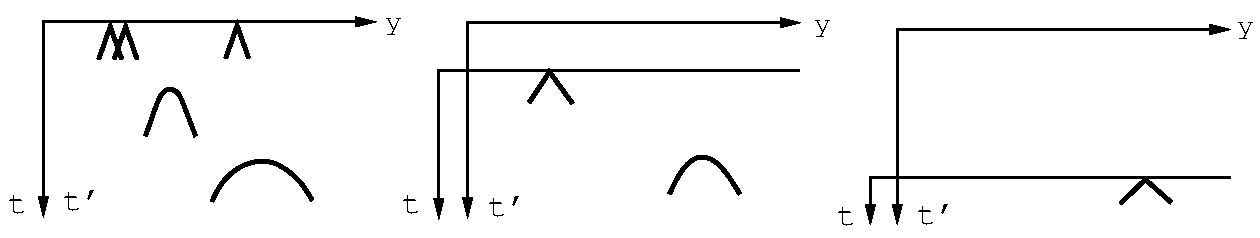
\includegraphics[width=0.65\textwidth]{vdmo/specz}
% \caption[specz]{测定速度的倾角谱方法。
% 为求出任何深度上的速度,只需在剖面的该神淙度上搜索出最陡倾角。在左图的地表面上,你可看到地
% 面的地滚波,其余两图表示逐步向下延拓时的状态,速度最慢的同相轴是波速逐次增大的双劭线之渐近线}
% \label{fig:vdmo/specz}
% \end{figure}
%
% \subsection{习题}
% \label{sec:3.5.11}
%
% \begin{enumerate}
% \item 设数据$P(y, h, t)$在中心点$y$变化时保持为恒定。如共中心点道集$P(h,t,z = 0)$
% 已知,根据双平方根方程
% \begin{equation*}
% \frac{\partial }{\partial z}P=-i\frac{\omega}{v}[\sqrt{1-(Y+H)^2}+\sqrt{1-(Y-H)^2}]P
% \end{equation*}
% 试定义一个能将$P(h,t,z = 0)$变换为$P(h=0, t, z)$的Stolt型积分变换。在利用Stolt偏
% 移时,应将你的答案按二维Fourier变换形式来表示。
%
% \item 根据互换性设有定义在正值和负值炮检距$h$上的一个CDP道集$u(h,t)$,试述下列诸
% 运算对它的影响:采用Fourier变换使之变换为$U(k_h, \omega)$;乘以$1 + sgn (\omega)
% sgn(k_h)$;再反向变换至$(h,t)$空间。
%
% \end{enumerate}
%
